%\title{emnlp 2017 instructions}
% File emnlp2017.tex
%

\documentclass[11pt,letterpaper]{article}
\usepackage{emnlp2017}

\usepackage{times}
\usepackage{latexsym}
 
% Uncomment this line for the final submission:
%\emnlpfinalcopy

%  Enter the EMNLP Paper ID here:
\def\emnlppaperid{***}

% Our packages
\usepackage{float}
\usepackage[font=small]{caption}
\usepackage{color}
\usepackage{graphicx}
\usepackage{booktabs}
\usepackage{subcaption}
\usepackage{hyperref}
\usepackage[utf8]{inputenc}
\usepackage{tabularx}
\usepackage{tablefootnote}
\usepackage{amsmath}
\usepackage{amssymb}
\usepackage{placeins}
\usepackage{scrextend}

\special{papersize=210mm,297mm}

%\usepackage{fixltx2e}

\newcommand{\todo}[1]{\textcolor{red}{TODO: #1}}
\newcommand{\edit}[1]{\textcolor{red}{#1}}
\newcommand{\bs}[1]{\textcolor{orange}{bs: #1}}

% To expand the titlebox for more authors, uncomment
% below and set accordingly.
% \addtolength\titlebox{.5in}    

%\title{Tell Me Why: Learning to Rank Answers and Their Justifications \todo{Jointly}}
\title{Tell Me Why: Using Question Answering as Distant Supervision for Answer Justification}


% Author information can be set in various styles:
% For several authors from the same institution:
% \author{Author 1 \and ... \and Author n \\
%         Address line \\ ... \\ Address line}
% if the names do not fit well on one line use
%         Author 1 \\ {\bf Author 2} \\ ... \\ {\bf Author n} \\
% For authors from different institutions:
% \author{Author 1 \\ Address line \\  ... \\ Address line
%         \And  ... \And
%         Author n \\ Address line \\ ... \\ Address line}
% To start a seperate ``row'' of authors use \AND, as in
% \author{Author 1 \\ Address line \\  ... \\ Address line
%         \AND
%         Author 2 \\ Address line \\ ... \\ Address line \And
%         Author 3 \\ Address line \\ ... \\ Address line}
% If the title and author information does not fit in the area allocated,
% place \setlength\titlebox{<new height>} right after
% at the top, where <new height> can be something larger than 2.25in

\date{}

\begin{document}

\maketitle

\begin{abstract}

For many applications of question answering (QA), being able to explain why a given model chose an answer is critical.  However, the lack of labeled data for  answer justifications makes learning this difficult and expensive.  Here we propose an approach that uses answer ranking as distant supervision for learning how to select informative justifications. 
We propose a neural network architecture for QA that reranks answer justifications as an intermediate (and human-interpretable) step in answer selection. Our approach is informed by a set of features designed to combine both learned representations and explicit features to capture the connection between questions, answers, and answer justifications.
 We show that with this end-to-end approach we are able to significantly improve upon a strong IR baseline in both justification ranking (+9\% rated highly relevant) and answer selection (+6\% P@1).  %We also provide an error analysis that demonstrates that we can use the justifications returned to better understand what our model has learned.
\end{abstract}

\section{Introduction}
\label{sec-emnlp2017:intro}

Developing interpretable machine learning (ML) models, that is, models where a human user can \emph{understand} what the model is learning, is considered by many to be crucial for ensuring usability and accelerating progress \cite{craven1996extracting,Kim2015MindTG, letham2015interpretable, Ribeiro2016WhySI}.  
% bs: removed for space, we talk more about this in related work
%As such, it has received much attention in recent years, especially as deep learning and complex architectures have seen dramatic gains in many tasks.
For many applications of question answering (QA), i.e., finding short answers to natural language questions, simply providing an answer is not sufficient. A complete approach must be interpretable, i.e., able to {\em explain} why an answer is correct. 
For example, in the medical domain, a QA approach that answers treatment questions would not be trusted if the treatment recommendation is not explained in terms that can be understood by the human user. 
%, the need for interpretable models:
%QA is one of the most challenging natural language understanding tasks~\cite{Etzioni:11}.  Adding to this challenge is the fact that, 
%for many applications of QA, simply providing an answer is not sufficient. A complete approach must also {\em explain} why an answer is correct. 
%For example, in the medical domain, a QA approach that answers treatment questions would not be trusted if the treatment recommendation is not explained in terms that can be understood by the human user. 
%Despite the importance of explanatory QA, the task of providing justifications as to \emph{why} the extracted answers are correct often takes a backseat to the accuracy of the system, and is not evaluated.
%is often overlooked and not evaluated. 

One approach to interpreting complex models is to make use of human-interpretable information % metric % ms: not a metric...
 generated by the model to gain insight into what the model is learning.  This can be an intermediate representation used by the model, as with the model-generated text spans of \citet{Lei2016RationalizingNP}, that serve as input to another classification network.  
By learning these intermediate representations end-to-end with a downstream task, they are optimized to correlate with what the model learns is discriminatory for the task, and they can be evaluated against what a human would consider to be important.
%\todo{need to define what a downstream task means to use this term}, they are optimized to correlate with what the model learns is discriminatory for the task, and they can be evaluated against what a human would consider to be important.
Here we apply this general framework for model interpretability to QA.
% ms: redundant with paragraph below
% propose a QA model that is able to provide free-text passages as justifications for the answers it selects.  

\begin{table}[t]
\begin{center}
\begin{footnotesize}
\begin{tabularx}{\linewidth}{p{0.13cm}p{6.8cm}}
\multicolumn{2}{p{8cm}}{\textbf{Question:} Which of these is a response to an internal stimulus?} \\
 (A) & A sunflower turns to face the rising sun. \\
 (B) & A cucumber tendril wraps around a wire. \\
 (C) &  A pine tree knocked sideways in a landslide grows upward in a bend. \\
 (\textbf{D}) &\textbf{Guard cells of a tomato plant leaf close when there is little water in the roots .} \\
\\
\multicolumn{2}{p{7.2cm}}{\textbf{Justification:} 
Plants rely on hormones to send signals within the plant in order to respond to internal stimuli such as a lack of water or nutrients. } \\

\end{tabularx}
\end{footnotesize}
\caption{{  Example of an 8th grade science question with a justification for the correct answer.  Note the lack of direct lexical overlap present between the justification and the correct answer, demonstrating the difficulty of the task of finding justifications using traditional distant supervision methods. }}
%space{-6mm} 
\label{tab:question_example}
\end{center}
\end{table}

In this work, we focus on answering multiple-choice science exam questions (Clark \citeyear{clark:2015}; see example in Table~\ref{tab:question_example}). 
This domain is challenging as: (a) approximately 70\% of science exam question shave been shown to require complex forms of inference to solve \cite{clark:2013,jansen-EtAl:2016:COLING}, and (b) there are few structured knowledge bases to support this inference.  
Within this domain, we propose an approach that learns to both select and explain answers, when the only supervision available is for which answer is correct (but not how to explain it).
%Within this domain, we propose an approach that jointly learns to select and explain answers, when the only supervision available is for which answer is correct (but not how to explain it) 
%\todo{PC's comment was remove reference to joint learning so it doesn't get us into trouble.  Do we need to say that we're learning the QA task while providing latent information for the explanation task?}. 
Intuitively, our approach chooses the justifications that provide the most help towards ranking the correct answers higher than incorrect ones.
More formally, our neural network approach alternates between using the current model with max-pooling to choose the highest scoring justifications for correct answers, and optimizing the answer ranking model given these justifications. %\todo{ms: tried to simplify, please check}
%bs - very good! thanks!
% scores all possible justifications for a chosen answer with the current model, and then uses max-pooling 
% re-ranks supporting textual evidence for a chosen answer then uses max-pooling 
%\todo{first reference to deep learning -- needs to be introduced before hand} 
%to choose the highest scoring justification and assign the score of the top-ranked justification to the answer candidate itself for use in the answer selection.  
%such that \todo{expand a bit; mention max-pooling?}.  
Crucially, these reranked texts serve as our human-readable answer justifications, and by examining them, we gain insight into what the model learned was useful for the QA task.   


The specific contributions of this work are:
\begin{enumerate}
\item We propose an end-to-end neural method for learning to answer questions and select a high-quality justification for those answers. 
Our approach re-ranks free-text answer justifications without the need for structured knowledge bases. 
%We formulate this such that the answer ranking supervises the justification re-ranking. 
With supervision only for the correct answers, % but not the quality of their corresponding justifications, % ms: redundant with previous text
we learn this re-ranking through a form of distant supervision -- i.e., the answer ranking supervises the justification re-ranking. 
%bs: I added detail in body of intro
%\todo{this is not very clear; say explicitly what we do with max pooling? or, actually, probably ok to remove since it's redundant to main body of the intro; better explain it there, and just summarize the novelty here}
%Because in our setup we have supervision only for the correct answers, but not for the corresponding answer justifications, .

\item We investigate two distinct categories of features in this ``little data'' domain: explicit features, and learned representations. % \todo{Deep learning jargon, needs to be introduced} \bs{I mainly diagree... and due to serious lack of space I can't intro... so idk.  mihai?}.  % ms: not necessary; well known in this community
We show that, with limited training, explicit features perform far better despite their simplicity. %\todo{Are they simpler? They were generated by a human carefully considering the data}.
%bs: i think we can support their simplicity --they're based on like, proportion of lexical overlap and IR scores.

\item We demonstrate a large (+9\%) improvement in generating high-quality justifications over a strong information retrieval (IR) baseline, while maintaining near state-of-the-art performance on the multiple-choice science-exam QA task, demonstrating the success of the end-to-end strategy.
%Importantly, our approach explains its selected answers significantly better than  a strong IR baseline, demonstrating the success of the joint strategy.
%We demonstrate near state-of-the-art performance on the multiple-choice science-exam QA task: our system would have placed 7th in a recent Kaggle challenge (top 4\%).\footnote{{\scriptsize \url{https://www.kaggle.com/c/the-allen-ai-science-challenge/leaderboard}}} 
%Further, our approach outperforms a recent model that relies on structured knowledge bases~\citep{khot2017tupleinf}, despite having a minimally-tuned, simple architecture, and a smaller set of text-only resources. 
% ms: I took it out because the natural question is why don't we evaluate on that dataset as well?
%which achieves state-of-the-art performance on a related question set. 
\end{enumerate}



%\todo{remove me later -- had weird splitting citation issue again.......... } 

%\todo{move this para to related work}

%The way we have formulated our justification selection (as a re-ranking of knowledge base sentences) is related to, but distinct from the task of answer sentence selection \cite[][inter alia]{Wang2010ProbabilisticTM, Severyn:12,Severyn:13a,Severyn:13b,Severyn2015LearningTR,wang2015long}.  Answer sentence selection is typically framed as a fully or semi-supervised task for factoid questions, and 
%.  Additionally, even when this isn't the case and a semi-supervised approach is necessary, 
%the problem is designed such that a correctly selected sentence will fully contain the answer text.
%the exact span of the answer is fully contained within the correct sentence.   
%Here, we have a variety of questions, many of which are non-factoid.  Additionally, we also have no direct supervision for our justification selection (i.e., we have no labels as to which sentences are good jutsifications for our answers), requiring a form of distant supervision where the performance on our QA task serves as our only signal as to whether or not we are selecting good jutstifcations.   Further, we are not actually looking for sentences that \emph{contain} the answer choice, as with answer sentence selection, but rather sentences which close the "lexical gap" \cite{Berger:00} between question and answer (as demonstrated in the question in Table \ref{tab:question_example}). 


%
%\todo{choose either ``explanation'' or ``justification'' and be consistent}
%\bs{i vote justification and tried to be consistent -- arguments? I'll leave the todo til the end to make sure we're good} 
%
%Question answering (QA), i.e., finding short answers to natural language questions, is one of the most challenging natural language understanding tasks~\cite{Etzioni:11}. Adding to this complexity is the fact that, for many applications of QA, simply providing an answer is not sufficient. A complete approach must also {\em explain} why an answer is correct. 
%For example, in the medical domain, a QA approach that answers treatment questions would not be trusted if the treatment recommendation is not explained in terms that can be understood by the human user. 
%Despite the importance of explanatory QA, the task of providing justifications as to why the extracted answers are correct is often overlooked and not evaluated. 
%
%In this work we argue that answers and their justifications re-enforce each other, and, thus, answer selection and justification should be addressed jointly.
%%bs: removed -- 2 ppl now think this is a bit of a jump/stretch
%%We see this as an initial step towards explainable artificial intelligence.\footnote{For more details see DARPA's Explainable Artificial Intelligence program: {\scriptsize \url{http://www.darpa.mil/program/explainable-artificial-intelligence}}.}
%In particular, we propose a joint approach to select and explain answers to multiple-choice science exam questions~\todo{cite ai2} by re-ranking supporting evidence in the form of free-text. The domain of science exam questions is challenging as: (a) many questions require natural language inference to be answered (see, for example, the question in Table~\ref{tab:question_example}) and (b) there are few structured knowledge bases to support this inference.  
%
%%Additionally, the task of selecting a justification for an answer in this domain is difficult because unlike in typical answer sentence selection tasks with factoid questions (where answer sentences generally completely contain the answer text)~\todo{cite moschitti}, here there is often a ``lexical chasm''~\cite{Berger:00} between answer choices and their justifications.  Also, answer sentence selection is typically a fully-supervised problem but here we have no labels for good justifications.
%The way we have formulated our justification selection (as a re-ranking of knowledge base sentences) is related to, but distinct from the task of answer sentence selection \cite[][inter alia]{Wang2010ProbabilisticTM, Severyn:12,Severyn:13a,Severyn:13b,Severyn2015LearningTR,wang2015long}.  Answer sentence selection is typically framed as a fully supervised task for factoid questions.  Additionally, even when this isn't the case and a semi-supervised approach is necessary, the problem is designed such that the answer is fully contained within the desired KB sentence.   Here, we have a variety of questions, many of which are non-factoid.  We also have no direct supervision for our justification selection, requiring a form of distant supervision (i.e., our joint-learning approach), and to further complicate the task, we are not specifically looking for sentences that \emph{contain} the answer choice, but rather sentences which close the "lexical gap" \cite{Berger:00} between question and answer (as demonstrated in the question in Table \ref{tab:question_example}). 

%Additionally, the task of selecting a justification for an answer in this domain is difficult because unlike in typical answer sentence selection tasks with factoid questions (where answer sentences generally completely contain the answer text)~\todo{cite moschitti}, here there is often a ``lexical chasm''~\cite{Berger:00} between answer choices and their justifications.  Also, answer sentence selection is typically a fully-supervised problem but here we have no labels for good justifications.

%\todo{reformulate -- our justs may or may not contain the answer - may be lexical chasm... not designed to contain the answer, but to address the lex chasm}


%Intro: Explanatory ML. Not �"black boxes". Here we focus on explainable QA. Selecting correct answers is important, but providing justifications as to why those answers are correct is critical in many domains.  This is often overlooked and not evaluated, and limits the ultimate utility and applicability of these systems.

%What we do: focus on science exam questions. hard for two reasons: ``lexical chasm'' which requires natural language inference to be solved. 
%We propose and evaluate an deep learning based approach that jointly extracts and explains answers. 

\section{Related work}

In many ways, deep learning has become the canonical example of the "black box" of machine learning and many of the approaches to explaining it can be loosely categorized into two types: approaches that try to interpret the parameters themselves (e.g., with visualizations and heat maps \citep{Zeiler2014VisualizingAU,nips15_hermann, Li2016VisualizingAU}, and approaches that generate a human-interpretable metric that is ideally correlated with what is being learned inside the model (e.g., \citet{Lei2016RationalizingNP}). Our approach falls into the latter type -- 
we use our model's reranking of human-readable justifications to give us insight into what the model considers informative for answering questions.  This allows us to see where we do well (Section \ref{sec-emnlp2017:justification_results}), and where we can improve (Section  \ref{sec-emnlp2017:erroranalysis}).

Deep learning has been successfully applied to many recent QA approaches and related tasks \cite[][inter alia]{Bordes2015LargescaleSQ,nips15_hermann, He2016CharacterLevelQA, dong2015question, Tan2016ImprovedRL}.
%are enticing, and for good reason -- many recent approaches to question answering and related tasks have had much success with various deep learning models \cite[][inter alia]{Bordes2015LargescaleSQ,nips15_hermann, He2016CharacterLevelQA, dong2015question, Tan2016ImprovedRL}.  
However, large quantities of data are needed to train the millions of parameters often contained in these models.  
%Of potentially greater utility in low-data domains, 
Recently, simpler model architectures have been proposed that greatly reduce the number of parameters while maintaining high performance \cite[e.g.,][]{Iyyer2015,chen2016thorough,Parikh2016ADA}.  
%For example, \citet{Iyyer2015}'s show that with their Deep Averaged Network, which replaces complex recurrent neural networks with an average of embeddings and a few, albeit large, dense layers, they improved performance on both a sentiment analysis and a QA task.  For natural language inference, \citet{Parikh2016ADA} used a simpler neural alignment  approach with an attention mechanisms to greatly reduce the size of their model while reaching then state-of-the-art performance.  
We take inspiration from this trend and propose a simple neural architecture for our task to offset the limited available training data. 

Another way to mitigate sparse training data is to include higher-level explicit features.  Like \citet{sachan2016science}, we make use of explicit features alongside features from distributed representations to capture connections between questions, answers, and supporting text.  However, we use a simpler set of features and while they use structured and semi-structured knowledge bases, we use only free-text.  %Additionally, though we also learn to select support from our knowledge base (in some ways similar to \citeauthor{sachan2016science}'s latent answer-entailing structure), since we are explicitly trying to perform \emph{explainable} question answering, here we evaluate the justifications learned by our approach and show that they are significantly better than a  strong IR baseline (Section \ref{sec-emnlp2017:justification_results}).   

Our approach to learning justification reranking end-to-end with answer selection is similar to the \citet{jansen2017framing} latent reranking perceptron,  which also operates over free text.  However, our approach does not require decomposing the text into an intermediate representation, allowing our technique to more easily extend to larger textual knowledge bases.  
%ir approach is able to aggregate information from a variety of sources into one justification, our light-weight approach however, does not rely on a large set of heuristics and heavy pre-processing to transform free-text into a structured knowledge base.  

The way we have formulated our justification selection (as a re-ranking of knowledge base sentences) is related to, but distinct from the task of answer sentence selection \cite[][inter alia]{Wang2010ProbabilisticTM, Severyn:12,Severyn:13a,Severyn:13b,Severyn2015LearningTR,wang2015long}.  Answer sentence selection is typically framed as a fully or semi-supervised task for factoid questions, where a correctly selected sentence fully contains the answer text.
%and the problem is designed such that a correctly selected sentence will fully contain the answer text.
Here, we have a variety of questions, many of which are non-factoid.  Additionally, we have no direct supervision for our justification selection (i.e., no labels as to which sentences are good justifications for our answers), motivating our distant supervision approach where the performance on our QA task serves as supervision for selecting good justifications.  Further, we are not actually looking for sentences that \emph{contain} the answer choice, as with answer sentence selection, but rather sentences which close the "lexical chasm" \cite{Berger:00} between question and answer (demonstrated in the example in Table \ref{tab:question_example}). 


%Related work: QA, multiple choice, kaggle challenge, explanation-centered inference, model-specific work (NNs, etc)

%Latest QA papers (latest trends, attn, etc)
%Inspired by this literature (cite DAN \& SNLI, simpler better), but we add this latent layer they don’t have (justification quality). For simple archs: see Danqi Chen at ACL 2016 (similar to DAN but for reading comprehension). 

%Attention models (ACL 2016). Simple especially when you don’t have enough data.

%(visualizations vs analysis of embeddings VS correlated metric EMNLP paper, etc -- interpreting wts if DL is impossible, rather, find correlations betw those and explanatory natural language)

 
%\todo{Add a paragraph comparing against the task of answer sentence selection (see that reviewer from CL, and all those kernel-based papers by Moschitti). The difference is that in our case the answer and its justification arrive from different sources (i.e., the answer is provided in the multiple-choice exam, whereas the justification is extracted from study guides), whereas in previous answer sentence selection work the answer is included in the sentence. In our case we have to deal with bigger ``lexical chasm'' between question/answer/justification.}

%\todo{Discriminative information retrieval for question answering sentence selection(Chen and Van-Durme): Presented a method that selects sentences which contain potential answers for questions from a very large corpus (10\^7 sentences, requiring several thousand questions for training). Their results are dramatically better than Lucene across two datasets and several evaluation measures.}
%(Yih et al.,2013; Wang and Manning, 2010; Heilman and Smith, 2010; Yao et al., 2013a) and recently using neural networks (Yu et al., 2014; Severyn and Moschitti,2015; Wang and Nyberg, 2015; Yin et al.,2016)

%Answer sentence selection diff because we don't need (or want?) complete answer inclusion.

%Our sentences being selected are unlabeled.

%TAG paper!!! 

\begin{figure}[t]
\begin{center}
\includegraphics[width=0.3\textwidth]{arch_overall.png}
\caption{ Architecture of our question answering approach.  
Given a question, candidate answer, and a free-text knowledge base as inputs, we generate a pool of candidate justifications, from which we extract feature vectors.  We use a neural network to score each and then use max-pooling to select the current best justification. This serves as the score for the candidate answer itself.  The red border indicates the components that are trained online. }
\label{fig:arch_overall}
\vspace{-5mm}
\end{center}
\end{figure}

\section{Approach}
\label{sec:approach}
One of the primary difficulties with the explainable QA task addressed here is that, while we have supervision for the correct answer, we do not have annotated answer justifications.  
Here we tackle this challenge by using the QA task performance as supervision for the justification reranking, allowing us to 
%extending a neural QA model to jointly learn both how to 
%jointly 
learn to choose both the correct answer and a compelling, human-readable justification for that answer.

Additionally, similar to the strategy Chen and Manning~\shortcite{chen2014fast} applied to parsing, we combine representation-based features with explicit features that capture additional information that is difficult to model through embeddings, especially with limited training data.
%second contribution is that, similar to the strategy Chen and Manning~\shortcite{chen2014fast} applied to parsing, we combine representation-based features with explicit features that capture additional information that is difficult to model through embeddings.



% ms: avoid "system" too engineering-y
The architecture of our approach is summarized in Figure \ref{fig:arch_overall}.  
Given a question and a candidate answer, we first query an textual knowledge base (KB) to retrieve a pool of potential justifications for that answer candidate.  
For each justification, we extract a set of features designed to model the relations between questions, answers, and answer justifications based on word embeddings, lexical overlap with the question and answer candidate, discourse, and information retrieval (IR) (Section \ref{sec:features}).
These features are passed into a simple neural network to generate a score for each justification, given the current state of the model.  A final max-pooling layer selects the top-scoring justification for the candidate answer and this max score is used also as the score for the answer candidate.  
The system is trained using correct-incorrect answer pairs with a pairwise margin ranking loss objective function to enforce that the correct answer be ranked higher than any of the incorrect answers. 

%The key here is that we use the current state of the model to select the best justification for a given answer candidate from a pool of many candidate justifications.  To do this, we modify the training procedure such that at the start of each epoch \todo{minibatch instead of epoch?}, we first compute a forward pass with each candidate justification to find the top-scoring justification for each candidate answer.
%For a given question, answer candidate, and justification, we combine features based on word embeddings, lexical overlap, discourse, and information retrieval (IR) together in a simple neural architecture to generate a score for the answer candidate.    We then use this selected justification to calculate our gradients for updating the model parameters.  

With this end-to-end approach, the model learns to select justifications that allow it to correctly answer questions.  We hypothesize that this approach enables the model to indirectly learn to choose justifications that provide good explanations as to why the answer is correct. We empirically test this hypothesis in Section \ref{sec:results}, where we show that indeed the model learns to correctly answer questions, as well as to select high-quality justifications for those answers. 
% ms: misleading; it reads as if answer selection is better than IR
% better than a strong IR baseline. 

\section{Models}
\label{sec-emnlp2016:models}

We use the extracted causal tuples to train three distinct distributional similarity models that explicitly capture causality. 

{\flushleft \textbf{Causal Embedding Model (cEmbed):}}
The first distributional similarity model we use is based on the skip-gram word-embedding algorithm of Mikolov et al.~\citeyear{mikolov2013distributed}, which has been shown to improve a variety of language processing tasks % \footnote{Chris Manning recently called embedding models the Sriracha sauce of NLP.} 
including QA~\cite{yih13,fried2015higher}.  In particular, we use the variant implemented by Levy and Goldberg~\citeyear{levy2014dependency} which modifies the original algorithm to use an arbitrary, rather than linear, context. 
Our novel contribution is to make this context task-specific: intuitively, the context of a cause is its effect. Further, these contexts are generated from tuples that are themselves bootstrapped, which minimizes the amount of supervision necessary.

The Levy and Goldberg model trains using single-word pairs, while our CMs could be composed of multiple words.  
For this reason, we decompose each cause--effect tuple, $(CM_c,CM_e)$, such that each word $w_c \in CM_c$ is paired with each word $w_e \in CM_e$. 

%so we decompose each cause--effect tuple, $(CM_c,CM_e)$, where each CM could be multi-word, into the Cartesian product of the words in CMs. such that each $w_c \in CM_c$ has as its context all $w_e \in CM_e$. 
After filtering the extracted cause-effect tuples for stop words and retaining only nouns, verbs, and adjectives, we generated over 3.6M $(w_c, w_e)$ word-pairs\footnote{For all models proposed in this section we used lemmas rather than words.} from the approximately 800K causal tuples.

The model learns two embedding vectors for each word, one for when the word serves as a target word and another for when the word serves as a context word.  Here, since the relation of interest is inherently directional, both sets of embeddings are meaningful, and so we make use of both -- the target vectors encode the effects of given causes, whereas the context vectors capture the causes of the corresponding effects. 


{\flushleft \textbf{Causal Alignment Model (cAlign):}}
Monolingual alignment (or translation) models have been shown to be successful in QA \cite{Berger:00,Echihabi:03,Soricut:06,Riezler:etal:2007,Surdeanu:11,yao2013}, and recent work has shown that they can be successfully trained with less data than embedding models~\cite{sharp2015spinning}. 
% Further, Fried et al.~\citeyear{fried2015higher} demonstrated that \todo{dest. distribution as semantic model of the source concept, which is important for our task as well.} % ms: nice, but no space

To verify these observations in our context, we train an alignment model that ``translates'' causes (i.e., the ``source language'') into effects (i.e., the ``destination language''), using our cause--effect tuples. 
This is done using IBM Model 1~\cite{Brown:93} and GIZA++~\cite{och03}. 
%We train an alignment model from our cause--effect tuples using  IBM Model 1~\cite{Brown:93} and GIZA++~\cite{och03}.


\begin{figure}[t!]
\begin{center}
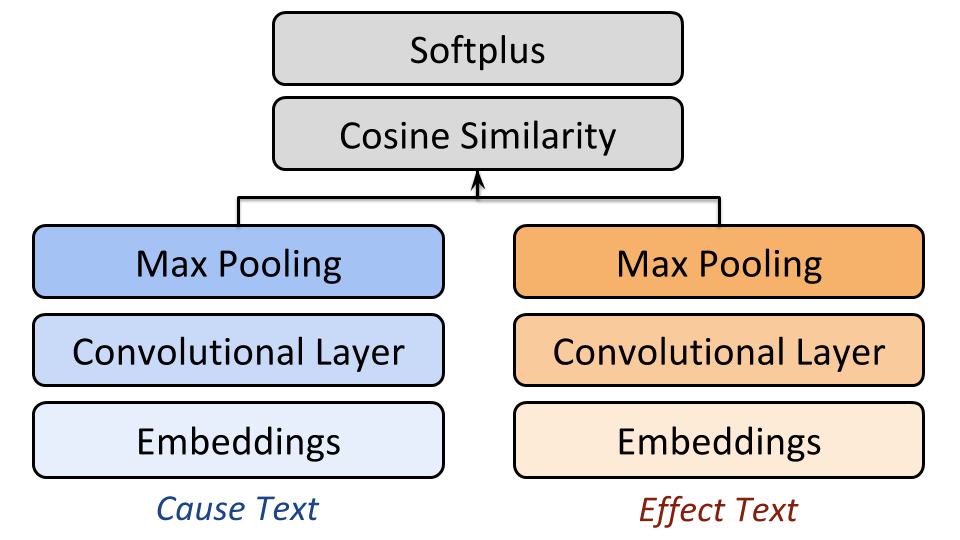
\includegraphics[width=0.7\textwidth]{mainmatter/emnlp2016-causal/cnn2.png}
%space{-2mm}
\caption{{\footnotesize Architecture of the causal convolutional network. }}
%space{-6mm}
\label{fig:cnn}
\end{center}
\end{figure}

{\flushleft \textbf{Causal Convolutional Neural Network Model (cCNN):}}
Each of the previous models have at their root a bag-of-words representation, which is a simplification of the causality task. To address this potential limitation, we additionally trained a convolutional neural network (CNN) which operates over variable-length texts, and maintains distinct embeddings for causes and effects.  The architecture of this approach is shown in Figure~\ref{fig:cnn}, and consists of two sub-networks (one for cause text and one for effect text), each of which begins by converting the corresponding text 
% (which has been padded to be of equal  length)  % ms: skip for now, until we understand it better
into 50-dimensional embeddings.  These are then fed to a convolutional layer,\footnote{The convolutional layer contained 100 filters, had a filter length of 2 (i.e., capturing bigram information), and an inner ReLU activation.} which is followed by a max-pooling layer of equal length.
Then, these top sub-network layers, which can be thought of as a type of phrasal embedding, are merged by taking their cosine similarity.  Finally, this cosine similarity is normalized by feeding it into a dense layer with a single node which has a softplus activation.  
In designing our CNN, we attempted to minimize architectural and hyperparameter tuning by taking inspiration from Iyyer et al.~\citeyear{iyyer2015deep}, preferring simpler architectures.
We train the network using a binary cross entropy objective function and the Adam optimizer~\cite{kingma2014adam}, using the Keras library~\cite{chollet2015keras} operating over Theano~\cite{2016arXiv160502688short}, a popular deep-learning framework.\footnote{We also experimented with an equivalent architecture where the sub-networks are implemented using long short-term memory (LSTM) networks~\cite{hochreiter1997long}, and found that they consistently under-perform this CNN architecture. Our conjecture is that CNNs perform better because LSTMs are more sensitive to overall word order than CNNs, which capture only local contexts, and we have relatively little training data, which prevents the LSTMs from generalizing well.}

{\flushleft \textbf{Noise-aware Causal Embedding Model (cEmbedNoise):}} 
We designed a variant of our cEmbed approach to address the potential impact of the noise introduced by our bootstrapping method.
While training, we weigh the causal tuples by the likelihood that they are truly causal, which we approximate with pointwise mutual information (PMI).
For this, we first score the tuples by their causal PMI and then scale these scores by the overall frequency of the tuple~\cite{riloff1996automatically}, to account for the PMI bias toward low-frequency items.  That is, the score $S$ of a tuple, $t$, is computed as: 

%space{-2mm}
%\scalebox{1.0}{
\begin{small}
\begin{equation}
S(t) = \log \frac{p(tuple|causal)}{p(tuple)} * \log (freq(tuple))
\end{equation} 
\end{small}
%}
%space{-2mm}

%Riloff~\citeyear{riloff1996automatically} propose a method for ranking their extracted patterns using $relevance\_rate * \log_2 (frequency)$.  As our relevance rate we use the pointwise mutual information of the extracted tuples, or $\log \frac{p(tuple|causal)}{p(tuple)}$, where $p(tuple| causal)$ is the ratio of the number of times that a given tuple is found in a causal construction versus any construction, and $p(tuple)$ is the frequency of the given tuple divided by the frequency of all the tuples. 
%Scaling the PMI by the frequency of the tuple mitigates its bias towards low-frequency items.
%we combine PMI with frequency information, so that we consider the likelihood of a pair to be causal to be:
%$p(causal|pair)$ \cite{riloff1996automatically}.
We then discretize these scores into five quantiles, ascribing a linearly decreasing weight during training to datums in lower scoring quantiles.%\footnote{\textcolor{blue}{We implemented this weighing process by repeating higher weight training examples more times.}}



%\section{Experiments and Evaluation}
%\label{sec:experiments}
%%\vspace{-2mm}
%
%We evaluate our approach at two levels.  First, we directly evaluate the quality of the embedding space in regards to the desired semantic relation.  Then, we evaluate the utility of the approach in an open-domain QA task.

\section{Direct Evaluation}
\label{sec:directeval}

To determine whether or not the proposed approach is able to capture the semantic relation of interest, causality, we replicate the quantitative evaluation of Levy and Goldberg~\citeyear{levy2014dependency}.  To demonstrate that their embeddings encoded functional similarity as opposed to topical similarity, they used their embeddings to rank a set of word pairs (each of which reflected one of the two types of similarity) using cosine similarity and showed that the word pairs which were functionally similar tended to be ranked higher than those with topical similarity.  Here, we do the same.

%\flushleft{\textbf{Data:}} 
\subsection{Data:}
We evaluate on a set of word pairs drawn from the SemEval 2010 Task 8 \todo{cite}, a multiway classification of semantic relations between nominals.  From the training set of this task, we used a total of XX nominal pairs, XX of which were cause-effect and XX which were randomly selected from the other XX relations.  This set was then randomly divided into equally-sized development and test partitions.

%\flushleft{\textbf{Baselines:}} 
\subsection{Baselines:}
We compared our embeddings against a standard \texttt{word2vec} model with a sliding window of XX as well as a random baseline where pairs were randomly shuffled. Additionally, we compared against a look-up baseline which counted the number of times a given nominal pair was found in the extracted cause-effect event database. 

\begin{table}[t!]
\begin{center}
%\begin{scriptsize}
\begin{footnotesize}
\begin{tabular}{ll}
\hline
\multicolumn{1}{l}{ Model } & \multicolumn{1}{l}{MAP} \\ %\multicolumn{1}{l}{Impr.} \\
%\cline{1-2}

\hline
%\multicolumn{2}{l}{\textit{Yahoo! Answers}} \\ % 185q (sent) ret=1p c=0.1 
%\hline
Random 			& 48.9 	\\
Lookup			& 93.1 	\\
Standard  		& 58.4	\\
Casual  			& 68.2*	\\

\end{tabular}
\end{footnotesize}
\caption{{\small Ability of each of the models and baselines to rank causal nominal pairs above non-causal pairs, as measured with mean average precision (MAP). Statistical significance (indicated by *) was determined through bootstrap resampling with 10,000 iterations.}}
\label{tab:MAP}
\end{center}
\end{table}
%MAP for Custom Vectors: 0.6816675505751166
%MAP for E2C Vectors: 0.6871338630607531
%MAP for Bidir Vectors: 0.6684350003582593
%MAP for Comparison (Baseline) Vectors: 0.5835158858435683
%MAP for Translation Model with lamda of 0.5 : 0.6156522257806402
%MAP for counting Matches: 0.9312613087523468
%MAP for Keras: 0.6752727545259546
%MAP for Random: 0.4892479543525109
%p < 0.01

\begin{figure}[t!]
\begin{center}
%\includegraphics[width=75mm]{rpcurves_all.png}
%\vspace{-4mm}
\caption{{\small Recall-precision curve showing the ability of each model to rank causal pairs above non-causal pairs. }}
\vspace{-6mm}
\label{fig:rpcurve_all}
\end{center}
\end{figure}

%\flushleft{\textbf{Results:}} 
\subsection{Results:}
In Table \ref{tab:MAP} we report the mean average precision (MAP) for each of the models and baselines.  The highest by far is for the look-up baseline.  However, this score is positively skewed by the fact that when pairs are found, there is extremely high confidence that they are of the relation of interest coupled with the fact that approximately 65\% of the pairs were not found in the database and so were all tied in last place.  As a consequence, there were far fewer average precisions to be combined when calculating the MAP, and most of the ones which were there had extremely high precision.  The MAP when using the customized vectors was significantly higher than that of the standard \texttt{word2vec} vectors (68\% versus 58\%), and both were higher than the baseline.  This suggests that while the standard implementation of \texttt{word2vec} encodes some causality information, our method encodes it far more directly. \todo{better word}.

\subsection{Discussion:}
We also examined the recall-precision curves for all models, shown in Figure \ref{fig:rpcurve}.  The curve for the customized vectors shows an atypical shape, where, despite the success of the customized vectors once recall reaches approximately 15\%, the highest ranked pairs (i.e. lower recall) had far \emph{worse} precision rather than higher precision.  To examine this, we analyzed the top-ranked 15\% of the pairs from the causal vectors.  

\todo{HEDGE THIS - more?}
Rather than finding that the high associations were due to noise in the training data, we found that the model appeared to be performing approximate inference, but here it was noisy inference.  For example, the top-ranked pair was (\emph{platform}, \emph{scaffold}) and there were no instances in the extracted causal events where \emph{platform} and \emph{scaffold} were found together in the same cause-effect pair.  

Instead, we found that there were only three extracted events with \emph{scaffold} in the effect text.  We checked to see if the words in the cause text of those events had other effect texts which overlapped lexically with \emph{platform}.  Indeed, we found the link illustrated in Figure \ref{fig:noisyinf}, where both \emph{platform} and \emph{malfunction} cause \emph{loss} thus bringing them closer together in the target embedding space, since they cause the same things.  This resulted in \emph{platform} being close to the effects of \emph{malfunction}, including \emph{scaffold}.  This demonstrates that the inference is influenced by frequency effects, as words like \emph{scaffold} and \emph{platform} are too infrequent to have robust representations in the embedding space.  

As this effect is entirely directional, we trained a set of vectors by reversing the input, such that the effects served as the targets and the causes were the contexts.  The recall-precision curve when using these embeddings to rank the SemEval pairs is shown in Figure \ref{fig:rpcurve_all}, labelled as E2C.  As expected, the curve follows that of the original vectors, as it suffers from the same issues, but with different noisy pairs ranked highly.  We then ranked the SemEval pairs using an average of the scores returned by the two causal embeddings, to mitigate the frequency effects.  That final, bidirectional curve is also shown in Figure \ref{fig:rpcurve_all}.
%Instead, we found that many of the causal events which whose cause argument contained the word \emph{platform} had effects which overlapped lexically with those whose cause arguments contained the word \emph{malfunction}, and that there w.  To illustrate, consider the following sentences 
%we had several extracted causal events whose cause contained the word \emph{platform} and whose effect contained the words \emph{}

\section{Indirect Evaluation}
\label{sec:indirecteval}

After having determined that the learned embeddings encoded causality, we designed an experiment to evaluate their utility in a down-stream task.  We chose question-answering (QA) as it has been shown that many questions require complex inference, including causality, in order to be explanably solved \todo{cite}.  

\subsection{Data:}
As we trained our embeddings using events extracted from open-domain resources, we chose to evaluate on a set of causal questions from Yahoo! Answers \todo{link}, hand-extracted with very simple surface patterns such as \emph{What causes ...}\todo{footnote with details?}.  There were a total of \todo{XX} questions, from which we used \todo{50\%} for training, \todo{25\%} for development, and \todo{25\%} for testing.
These questions were filtered such that each had at least four candidate answers
\todo{detail about the avg num answers, etc}

\subsection{Experimental Design:}
We evaluate the contribution of the causal embeddings model using the standard reranking architecture \todo{cite} of \todo{cite naacl and peters acl}.
%In pilot experiments, we found that aligning only nouns, verbs, adjectives, and adverbs yielded higher performance. TALK ABOUT?
In this architecture, the candidate answers are initially ranked using a shallow candidate retrieval (CR) component, then they are re-ranked using the model features along with the CR score. 
We used SVM rank\todo{cite/link}, a Support Vector Machine adapted for ranking, for our learning framework.
We compare the performance of the causal embeddings model against the same standard skipgram model used in Section \ref{sec:directeval}.
As features, we use the same set as \todo{cite naacl and acl}: the maximum and average pairwise cosine similarity between question and answer words, as well as the overall similarity between the composite question and answer vectors.  When using the causal embeddings however, we first determine (through lexical pattern matching) whether the question text is the cause or the effect, thus determining which embeddings to use for the question and candidate answer texts.  For example, in a question such as "Q: What causes X? A: Y", the cosine similarities would be found using the effect vectors for the question words and the cause vectors for the answer candidate words. \todo{good grief, redo this}   


\section{Experiments}
\label{sec:experiments}

\subsection{Data}
\label{sec:data}


{\flushleft {\bf Questions:}} We assembled a corpus of 1,000 third to fifth grade standardized elementary school science exam questions, consisting of 346 publicly available questions gathered from standardized exams in 12 states, as well as 654 closed questions from an exam generating service. 
All questions are multiple choice with four possible answer candidates. Questions vary in length from 1 to 6 sentences, while the four multiple choice answer candidates are generally either single words or short phrases. 
Because of the small size of this corpus, our models were evaluated using 5-fold crossvalidation, with 3 folds for training, one for development, and one for test. 

{\flushleft {\bf Knowledge bases:}} Sentences from six text resources served as input for TAG generation.  Five of these resources are in the science domain and include two state-specific science exam study guides, a teacher's manual, a children's science dictionary, and a set of exam review flashcards.  Each of these in-domain resources was selected to be at a third-to-fifth grade knowledge level, and contained between 283 and 1,314 sentences (for a total of 3,832 in-domain sentences).  
The Simple Wiktionary\footnote{\url{http://simple.wiktionary.org}} was included as a large open-domain dictionary resource written at knowledge level similar to that of the exam questions.  Starting with over 24,000 definitions, we filtered these to include only definitions for nouns, verbs, and adjectives, for a total of 17,473 sentences after filtering.

\subsection{Tuning}
\label{sec:tuning}
We tuned the following hyperparameters once on the development data to optimize both performance and stability.

{\flushleft \textbf{Number of candidate justifications:}} 
Each of the multiple choice answers can have a large number of candidate justifications.  To reduce runtime and assist learning, we filter this initial list of TAGs to include only a subset of TAGs with a high focus word mass. We kept all justifications tied for focus mass with the justification in 25th place, resulting in a variable number of TAGs for each QA pair.  For our dataset, the mean number of TAGs for each QA pair was 141. \\

{\flushleft \textbf{Perceptron Hyperparameters:}} We investigated the perceptron hyperparameters using a coarse grid search and found a stable optimum with 10 epochs, a $\tau$ of 1.0, burn in of 5 epochs (i.e., the weight updates were not added to the average weights for the first five epochs), and a learning rate (which dampened the updates to the weight vector) of 0.1. Since model results can vary depending on the random seed used for initialization, rather than using a single perceptron we use an ensemble of 50 perceptron models initialized with random weights.  These models are combined in a simple voting scheme, where each model casts a single vote for each question (distributing the vote only in the case of ties).\\

{\flushleft \textbf{Feature Normalization:}} To minimize the effect of outliers in the feature space, we log-transformed the feature values, and then rescaled each feature independently to lie within the range of $-1$ to $1$, using the formula
\mbox{$normalized  = lower + (original - min)\frac{(upper - lower)}{(max - min)}$},
where $upper$ and $lower$ are the desired boundaries for the normalization ($1$ and $-1$, respectively), $max$ and $min$ are the maximum and minimum values for the corresponding feature across the training dataset, and $normalized$ is the result of normalizing $original$.
Note that during testing it is possible to see feature values outside of their known $[min, max]$ interval, which means that after normalization their values will fall outside the $[-1, 1]$ interval. We do not do any additional post-processing for these values.


\subsection{Baselines}
\label{sec:baselines}

We include the following baselines: 

{\flushleft {\bf Random:}} selects an answer randomly.
{\flushleft {\bf Candidate retrieval (CR):}} ranks answers using an approach similar to the baseline model in Jansen et al.~\citeyear{jansen14}, which uses features that measure cosine similarity over {\em tf-idf} vectors (e.g., Ch. 6, Manning et al.\citeyear{manning08}) to rank answer candidates in a ``learning to rank'' (L2R) framework.  
Traditionally, with retrieval systems, short answers to questions are dynamically constructed from larger parent documents, and the top-scoring answer (defined as the answer with the highest {\em tf-idf} score between that answer candidate and a query vector made from the question) is taken to be the winner.  Here we adapt this setup to multiple choice exams by: (a) using query vectors that contain words from both the question and multiple choice answer candidate, and (b) generating features from the top {\em tf-idf} score for each answer candidate in a given question, which are then combined in the learning-to-rank framework.  We then take the short passage retrieved by the system as a justification for why that answer candidate is correct. 

Documents are constructed across the six knowledge bases by dividing each corpus by subsection (for texts), by definition (for dictionaries), or by flashcard.  We implemented the document indexing and retrieval system using Lucene\footnote{\url{http://lucene.apache.org}}.  Each sliding window of $N$ sentences in a given document served as a potential answer justification. Using the development questions, we empirically determined that a two-sentence window performed best, though performance did not significantly differ for window sizes between one and five sentences.  This  model generates two features: a cosine similarity score between the query vector and the best-scoring candidate answer justification in a given corpus, and a linear model that combines this cosine similarity with the cosine similarity between the query vector and the entire document, blending both local (answer justification) and global (document) context. 

Because our six corpora are of different genres (study guide, teachers guide, dictionary, flashcards), domains (science-domain vs. open-domain), and lengths (300 to 17,000 sentences), we implement six separate {\em tf-idf} models, each containing documents only from a single corpus. We then combine the two retrieval features from each model (12 features total) into a ranking perceptron \cite{Shen:Joshi:2005,Surdeanu:11} to learn which knowledge bases are most useful for this task.  This ensemble retrieval model produces a single score for each multiple choice answer candidate, where the top-scoring answer candidate is selected as the winner.  The top-scoring answer justifications from each of the six retrieval models then serve as justifications. 


 
{\flushleft {\bf Jansen et al. (2014):}} the best-performing combined lexical semantic (LS) and CR model of Jansen et. al~\citeyear{jansen14}, which was shown to perform well for open domain questions.  Similar to the CR model, we adapted this model to our task by including six separate recurrent neural network language models (RNNLM) of Mikolov et al.\citeyear{mikolov13,mikolov10}, each trained on one of the six knowledge bases.  Two features that measure the overall and pairwise cosine similarity between a question vector and multiple choice answer candidate vector are included.  The overall similarity is taken to be the cosine similarity of the composite vectors of both the question and answer candidate, obtained by summing the vectors for the individual words within either the question or answer candidate vectors, then renormalizing these composite vectors to unit length.  The pairwise similarity is computed as the average pairwise cosine similarity between each word in the question and answer candidate.  Two features from each of the six LS models are then combined with the two features from each of the CR models (24 features total) as above using a ranking perceptron, with the top-scoring answer candidate taken as correct.  Because the LS features do not easily lend themselves to constructing answer justifications, no additional human-readable justifications were provided by this model. 


\subsection{Results}
\label{sec:results}

Here we first investigate the performance of two variants of the TAG model with respect to justification length.  We then compare the best-performing model with the baselines, and show that the TAG and CR models can be combined to increase performance. We use the standard implementation for precision at 1 (P@1) ~\cite{manning08} and a tie-aware implementation of mean reciprocal rank (MRR) \cite{mcsherry2008}.



%
% Performance versus path length
%
\begin{table}[t]
\caption{{
Performance as a function of justification length in sentences (or, the number of graphlets in a TAG) for two models: one aware of connection-type, and one that is not. Bold font indicates the best score in a given column for each model group. 
}}
\small
\begin{center}
%\begin{tabular}{p{0.3mm}p{55mm}llll}
\begin{tabular}{lllll}
\multicolumn{1}{l}{ } & \multicolumn{1}{l}{ } & \multicolumn{1}{l}{P@1} & \multicolumn{1}{l}{ } & \multicolumn{1}{l}{MRR} \\
\multicolumn{1}{l}{ Model } & \multicolumn{1}{l}{P@1} & \multicolumn{1}{l}{Impr.} & \multicolumn{1}{l}{MRR} & \multicolumn{1}{l}{Impr.} \\
\hline
\multicolumn{5}{l}{Normal}\\
\hline
1G					& 35.33			& --				& 59.26  		&	--  \\
2G					& {\bf 38.16}	& {\bf 8.0\%}	& {\bf 61.33}  	&	{\bf 3.5\%}  \\
3G					& 37.78			& 6.3\%			& 61.14  		&	3.2\%  \\
\\
\hline
\multicolumn{5}{l}{Connection-type aware (Daum{\'e})}\\
\hline
1G\textsubscript{CT}			& 34.80			& --				& 58.86  		& --  \\
2G\textsubscript{CT}			& {\bf 39.91}	& {\bf 14.7\%}	& {\bf 62.53}  	& {\bf 6.2\%} \\
3G\textsubscript{CT}			& 38.53			& 10.7\%			& 61.65  		& 4.7\%  \\

\hline
\end{tabular}

\vspace{-6mm}
\label{tab:pathlength}
\end{center}
\end{table}


\subsubsection{Justification Length}
\label{sec:pathlength}
Table~\ref{tab:pathlength} shows the performance of the TAG model as a function of increasing justification length.
Here, the $k$G models contain exclusively justifications of length $k$ (we explore TAGs of varying length later in this section).
Short two-sentence (or two-graphlet) TAGs significantly outperform single sentence TAGs, with single sentence (1G) TAGs starting at 35.3\% P@1, increasing to 38.2\% for two-sentence (2G) TAGs, hen decreasing slightly to 37.8\% for three-sentence (3G) TAGs. 
In previous work, we observed that for a variety of word-level graphs and traversal algorithms, QA performance tends to rapidly peak when aggregating two or three words, then slowly decreases as more words are aggregated due to ``inference drift'' in the graph 
traversal process
(i.e., following the connections from \emph{breakfast} $\rightarrow$ \emph{hashbrowns} $\rightarrow$ \emph{potato} $\rightarrow$ \emph{field} would potentially connect questions about breakfast to information about potato or even soccer fields)   \cite{fried2015higher}.  

Though our sentence aggregation model contains far more structure than the higher-order lexical semantic graphs of Fried et al. ~\citeyear{fried2015higher}, and is represented at the level of the sentence or graphlet rather than individual lemmas, we hypothesize based on this previous work that we may be observing the beginning of same characteristic peak in performance reported there.  Because runtime increases exponentially with the number of sentences included in a TAG, it quickly becomes intractable to test this with TAGs containing more than 3 graphlets. 

Extending the model to include a knowledge of the connection type (or the type of lexical overlap, see Section~{\ref{sec:characterizing}) between sentences in a given TAG using Daum{\'e}'s method~\cite{daume2007} increases performance, suggesting that different kinds of connections are best identified through different feature patterns.  Here, the connection-type aware 2G\textsubscript{CT} model outperforms the regular 2G model by nearly 2\% P@1 (absolute), increasing performance to 39.9\% -- an increase of +14.7\% (relative) over using only single-sentence TAGs.\footnote{Each of the 50 models in the ensemble reranker is initialized with random weights, causing the small performance difference between 1G and 1G\textsubscript{CT}}





\subsubsection{Combined Models}
\label{sec:combinedmodels}
%
% Combined model performance
%
\begin{table*}[t]
    \small
    \caption{{
Performance of the baseline and best-performing TAG models, both separately and in combination. TAG justifications of different short lengths were found to best combine in single classifiers (denoted with a $+$), where models that combine the CR baseline or long (3G) TAG justifications best combined using voting ensembles (denoted with a $\cup$). Bold font indicates the best score in a given column for each model group. Asterisks indicate that a score is significantly better than the highest-performing baseline model (* signifies $p < 0.05$, ** signifies $p < 0.01$).  The dagger indicates that a score is significantly higher than the score in the line number indicated in superscript ($p < 0.01$). All significance tests were implemented using one-tailed non-parametric bootstrap resampling using 10,000 iterations. }}
\begin{center}
\begin{tabular}{p{0.3mm}p{55mm}llll}
\multicolumn{1}{l}{ } & \multicolumn{1}{l}{ } & \multicolumn{1}{l}{ } & \multicolumn{1}{l}{P@1} & \multicolumn{1}{l}{ } & \multicolumn{1}{l}{MRR} \\
\multicolumn{1}{l}{\#} & \multicolumn{1}{l}{ Model } & \multicolumn{1}{l}{P@1} & \multicolumn{1}{l}{Impr.} & \multicolumn{1}{l}{MRR} & \multicolumn{1}{l}{Impr.} \\

\hline
& \multicolumn{5}{l}{Baselines }\\
\hline
1 & Random					& 25.00 			& --		& 52.08  		& --	  \\
2 & CR 						& {\bf 40.20} 	& -- 	& {\bf 62.49}	&	--  \\
3 & Jansen et al. (2014)		& 37.30 			& --		& 60.95 			& 	--	 \\

\\
\hline
& \multicolumn{5}{l}{Combined models with justifications of variable lengths (Single classifier)}\\
\hline
4 & 1G + 2G										& 38.69			& --		& 61.43  	& --  \\
5 & 1G\textsubscript{CT} + 2G\textsubscript{CT} 	& {\bf 42.88$\dagger ^4$}	& {\bf +6.7\%}		& {\bf 63.94\%}  	& {\bf +2.3\%}	  \\

\\
\hline
& \multicolumn{5}{l}{Combined models that include the CR baseline (Voting)}\\
\hline
6 & CR $\cup$ 1G\textsubscript{CT} $\cup$ 2G\textsubscript{CT} $\cup$ 3G\textsubscript{CT} 			& 43.15*			& +7.3\%			& 64.51*		& +3.2\%	  \\
7 & CR $\cup$ (1G\textsubscript{CT} + 2G\textsubscript{CT}) $\cup$ 3G\textsubscript{CT} 			& {\bf 44.46**}		& {\bf +10.6\%}		& {\bf 65.53**} 		& {\bf +4.9\%}	  \\

\hline
\end{tabular}
\vspace{-6mm}
\label{tab:combinedmodels}
\end{center}
\end{table*}

Where Table~\ref{tab:pathlength} lists models that contain justifications of static length, Fried et al.~\citeyear{fried2015higher} showed that combining paths of different lengths into a single classifier can increase performance.  The performance of TAG models that combine justifications of different lengths, as well as the baseline models, is shown in Table~\ref{tab:combinedmodels}.

{\flushleft {\bf Baselines:}} Where the lexical semantics model of Jansen et al. ~\citeyear{jansen14} outperformed their CR baseline by +36\% (relative) on a large corpus of open-domain questions from Yahoo Answers, here on elementary science exams, the lexical semantic features decrease performance.  Our conjecture is that the performance difference is due to the difference in the size of the corpora used to train the lexical semantic model -- where Jansen et al. trained their lexical semantic model using Gigaword, here we are limited by the relatively small size of our text resources.  Jansen et al. ~\citeyear{jansen14} reported that a domain-specific version of their lexical semantic model performed poorly when trained on a biology textbook and subset of Wikipedia, and others have since shown that lexical semantic models perform poorly with small amounts of training data \cite{sharp-EtAl:2015:NAACL-HLT}. 

{\flushleft {\bf Combined Models:}} Single-classifier models containing both 1G and 2G TAGs were generated for both the normal and connection-type-aware models.  The 1G + 2G model performs only slightly better than 2G alone, but when the models are connection-type aware, there is greater benefit to combining the different path lengths -- the connection-type-aware 1G\textsubscript{CT} + 2G\textsubscript{CT} model (line 5) increases performance to 42.9\% P@1 (compare to the static-length 2G\textsubscript{CT} performance of 39.9\%).


As the CR baseline and the TAG models are performing inherently different tasks (information \emph{retrieval} and information \emph{aggregation} respectively), we are able to combine them together in a voting model in order to create a full system that contains the benefits of each.
The voting models that incorporate both the CR baseline and TAG models across all justification lengths are included on lines 6 and 7.  Both models significantly increase performance over the CR baseline, with the voting model that couples 1G\textsubscript{CT} + 2G\textsubscript{CT} as a single classifier (and single vote) performing better than when 1G\textsubscript{CT} and 2G\textsubscript{CT} vote separately.  This best-performing model reaches 44.5\% P@1, increasing performance over the CR baseline by +10.6\% (relative). %All in all
This set of experiments demonstrates that our approach of jointly ranking answers and justifications is complementary to a strong information retrieval baseline, and significantly improves performance at the task of selecting the correct answer.  


\subsubsection{Justifications}


%
% Justification example (IR)
%
\begin{table*}[t]
\caption{{ \label{font-table} Example justifications from the CR baseline and their associated ratings. }} %  (N=20, c=0.1)
\begin{center}
\begin{footnotesize}
%\begin{tabular}{lcc}
%\cline{2-3}
%\begin{tabular}{cl}
\begin{tabularx}{\textwidth}{p{1cm}p{11.5cm}}
%\multicolumn{1}{r}{} & \multicolumn{1}{l}{} \\
%\cline{1-2}
%\hline
\hline
\multicolumn{1}{c}{} & \multicolumn{1}{c}{Question} \\
\hline			
\multicolumn{2}{l}{	What is the interaction between the producer and the consumer in a food chain?} \\
		&	\textbf{[A] The consumer eats the producer for energy.}  \\
		&  [B] The consumer does not interact directly with the producer. \\
			&   [C] The producer eats other producers for energy.   \\
			& [D] The producer eats the consumer for energy. \\
%Answer		&	The consumer eats the producer for energy. \\			

\multicolumn{1}{c}{} & \multicolumn{1}{c}{} \\				
\hline
\multicolumn{1}{l}{Rating} & \multicolumn{1}{c}{Example Justification} \\
\hline			
{\em Good }		&	A primary (1st) consumer eats producers (plants). A secondary (2nd) consumer eats primary consumers. {\em [Barrons SG]}  	\\
{\em Half }		&	The food chain starts with a producer (a plant) and ends with a decomposer. {\em [Flashcards]} \\
{\em Topical }	&   A herbivore is an organism that depends on plants for most of its food and energy. {\em [Science Dictionary]} \\
{\em Offtopic }	&	When a plate moves suddenly a great amount of energy is released.  These waves cause damage...  {\em [Virginia SG]} \\
%\end{tabular}
\end{tabularx}
\end{footnotesize}
\label{tab:justificationsIRexamples}

\end{center}
\end{table*}


%
% Justification example (TAG)
%
%\begin{figure}[t!]
%\begin{center}
%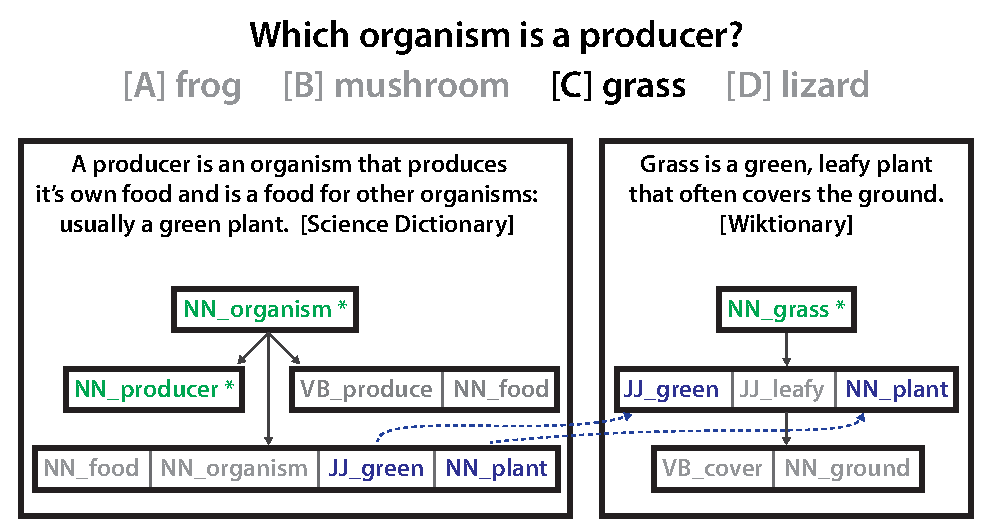
\includegraphics[width=75mm]{example_tig_producer2.pdf}
%\vspace{-2mm}
%\caption{ An example TAG path and justification rated as {\em good}. \note{TODO: Redraw figure with different line widths, closer to the original DOT file?}}
%%\caption{{\small An example of the alignments produced by the two discourse models.  The sequential model aligns pairs of consecutive sentences, capturing intersentence associations such as \emph{cider--apples}, and \emph{orchard--autumn}.  The RST model generates alignment pairs from participants in all (binary) discourse relations, capturing both intrasentence and intersentence alignments, including 
%%\emph{apples--orchard, cider--apples}, and \emph{cider--autumn}.}}
%% ms: I get the point, but there is value in brevity. Plus, maybe we should not use Bob as example :)
%%the intersentence alignments above along with intrasentence and multi-sentence alignments, including \emph{Bob--cider, apples--orchard}, and \emph{cider--autumn}.}}
%\vspace{-5mm}
%\label{fig:justificationTAGexample}
%\end{center}
%\end{figure}



\begin{table}[]
\small
\caption{{An example TAG and justification rated as {\em good}.  The two sentences connect on non-focus "other" shared words (e.g., \emph{green, plant}) which are not found in the question or answer, but which are highly related to the focus words. }} 
\begin{tabularx}{\textwidth}{p{2.5cm}p{11cm}}
%\hline
%\multicolumn{2}{l}{EXAMPLE: Other} \\
\hline
% Question Info
Question & Which organism is a producer? (GR:5)     \\
Focus Word(s) &   (NN\_producer, 0.92) (NN\_organism, 0.08) \\
Answers & (A) frog  (B) mushroom   (C) grass    (D) lizard \\
\hline
% Correct Answer Info
Correct Answer &  grass \\
Focus Word(s) &   (NN\_grass, 1.00) \\
\multicolumn{2}{c}{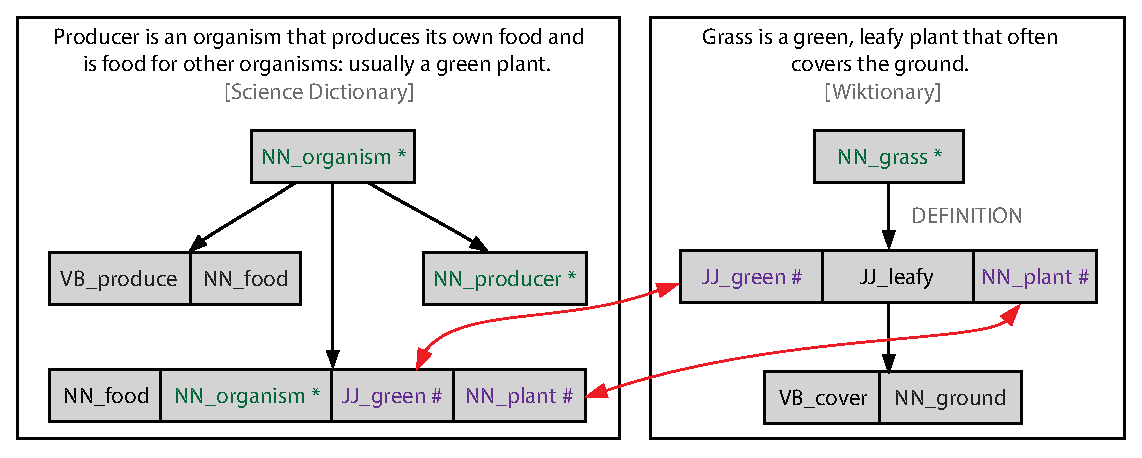
\includegraphics[width=115mm]{tag_good_justification.pdf}}
\\
\hline
\end{tabularx}
\label{ex:tagQsXs}
\end{table}






%
% Justification Examples - EXTRA
%
%\begin{table}[]
%\caption{{  Example of a TAG {\bf connected on answer focus} words. }} 
%\begin{tabularx}{\textwidth}{p{2.5cm}p{11cm}}
%%\hline
%%\multicolumn{2}{l}{EXAMPLE: Other} \\
%\hline
%% Question Info
%Question & What are the stages of development of an organism called? (GR:5)   \\
%Focus Word(s) &  (NN\_organism, 0.80) (NN\_stage, 0.13) (NN\_development, 0.07) \\
%\hline
%% Correct Answer Info
%Correct Answer &  Life cycle \\
%Focus Word(s) &  (NN\_cycle, 0.92) (NN\_life, 0.08) \\
%\multicolumn{2}{c}{\includegraphics[scale=0.5]{q58a1p2363connection.png}}\\
%\hline
%\end{tabularx}
%\label{ex:tagAns}
%\end{table}

%\begin{table}[]
%\caption{{  Example of a TAG {\bf connected on question and answer focus words}. (Somewhat more challenging focus word extraction, but we end up matching most of the words).  }} 
%\begin{tabularx}{\textwidth}{p{2.5cm}p{11cm}}
%%\hline
%%\multicolumn{2}{l}{EXAMPLE: Other} \\
%\hline
%% Question Info
%Question & Different types of organs that work together to perform a specific life function are called a(n) \_\_\_. (GR:5)   \\
%Focus Word(s) &   (VB\_work, 0.23) (VB\_perform, 0.23) (NN\_n, 0.23) (RB\_together, 0.09) (NN\_life, 0.07) (JJ\_specific, 0.06) (JJ\_different, 0.04) (NN\_function, 0.03) (NN\_organ, 0.01) \\
%\hline
%% Correct Answer Info
%Correct Answer &  organ system \\
%Focus Word(s) &   (NN\_system, 0.67) (NN\_organ, 0.33) \\
%\multicolumn{2}{c}{\includegraphics[scale=0.5]{q61a2p1104connection.png}}\\
%\hline
%\end{tabularx}
%\label{ex:tagQuest+Ans}
%\end{table}

%\begin{table}[]
%\caption{{  Example of a TAG connected only on answer focus words. Despite a non-ideal ranking of the question focus words, the system is able to lock onto this as a good justification of the correct answer.}} 
%\begin{tabularx}{\textwidth}{p{2.5cm}p{11cm}}
%%\hline
%%\multicolumn{2}{l}{EXAMPLE: Other} \\
%\hline
%% Question Info
%Question & Pots and pans are most often made from metal because \_\_\_. (GR:5)     \\
%Focus Word(s) &   (NN\_pot, 0.48) (NN\_pan, 0.48) (NN\_metal, 0.04) \\
%\hline
%% Correct Answer Info
%Correct Answer &  metals conduct heat well \\
%Focus Word(s) &   (NN\_heat, 0.44) (RB\_well, 0.44) (NN\_metal, 0.07) (VB\_conduct, 0.04) \\
%\multicolumn{2}{c}{\includegraphics[scale=0.5]{q100a3p908connection.png}}\\
%\hline
%\end{tabularx}
%\label{ex:tagXs}
%\end{table}

%\begin{table}[]
%\caption{{  {\bf Error example: Construction and Ranking vs Answer Selection:} Example of a question which requires {\bf complex inference}.  Our system aggregate sentences by connecting on {\bf question focus words as well as non-focus words}, to construct a good justification for the correct answer and rank it to the top of the justifications for that answer candidate. }} 
%\begin{tabularx}{\textwidth}{p{2.5cm}p{11cm}}
%%\hline
%%\multicolumn{2}{l}{EXAMPLE: Other} \\
%\hline
%% Question Info
%Question & In a food chain or web, the most efficient users of the Sun's energy are \_\_\_. (GR:5)     \\
%Focus Word(s) &   (NN\_chain, 0.23) (NN\_web, 0.23) (NN\_user, 0.22) (NN\_energy, 0.22) (NN\_food, 0.05) (NN\_sun, 0.03) (JJ\_efficient, 0.02) \\
%\hline
%% Correct Answer Info
%Correct Answer &  herbivores \\
%Focus Word(s) &   (NN\_herbivore, 1.00) \\
%\multicolumn{2}{c}{\includegraphics[scale=0.5]{q67a2p1connection.png}}\\
%\hline
%\end{tabularx}
%\label{ex:tagQsXsWrong}
%\end{table}
%
%
%\begin{table}[]
%\caption{{  {\bf Error example:} A similar example to the last one -- much of the time we're able to construct and rank very good TAGs (for a given answer candidate), but the last step -- selecting the best justification, is more sensitive to {\emph well connected answers} rather than {\emph good answers}.  Here the two aggregated sentences are {\bf connected on question focus words.}  }} 
%\begin{tabularx}{\textwidth}{p{2.5cm}p{11cm}}
%%\hline
%%\multicolumn{2}{l}{EXAMPLE: Other} \\
%\hline
%% Question Info
%Question & All organisms need food to survive. Which statement best describes the purpose of food for organisms? (GR:4)    \\
%Focus Word(s) &   (NN\_organism, 0.34) (NN\_organism, 0.34) (VB\_survive, 0.08) (NN\_food, 0.05) (VB\_need, 0.03) (NN\_food, 0.08) (NN\_purpose, 0.05) (NN\_statement, 0.03) \\
%\hline
%% Correct Answer Info
%Correct Answer &  Food provides energy for growth. \\
%Focus Word(s) &   (NN\_energy, 0.68) (NN\_growth, 0.16) (VB\_provide, 0.11) (NN\_food, 0.05) \\
%\multicolumn{2}{c}{\includegraphics[scale=0.5]{q19a3p2833connection.png}}\\
%\hline
%\end{tabularx}
%\label{ex:tagQsAsWrong}
%\end{table}
%
%
%
%\begin{table}[]
%\caption{{ {\bf Error example:} Another example of {\bf complex inference} that {\bf connects on other words}, in this case {\emph river}.  Again we're ranking this \todo{path} to the candidates for a given answer, but not selecting it out of the 4 multiple choice answers.  }} 
%\begin{tabularx}{\textwidth}{p{2.5cm}p{11cm}}
%%\hline
%%\multicolumn{2}{l}{EXAMPLE: Other} \\
%\hline
%% Question Info
%Question & Moving water was the most important factor in forming which of these? (GR:5)   \\
%Focus Word(s) &   (VB\_move, 0.68) (NN\_factor, 0.16) (NN\_water, 0.11) (JJ\_important, 0.05) \\
%\hline
%% Correct Answer Info
%Correct Answer &  the Grand Canyon \\
%Focus Word(s) &   (NN\_canyon, 0.67) (NN\_grand, 0.33) \\
%\multicolumn{2}{c}{\includegraphics[scale=0.5]{q33a0p57connection.png}}\\
%\hline
%\end{tabularx}
%\label{ex:tagXsWrong}
%\end{table}

The previous experiments demonstrate that our method performs well at identifying correct answers. But how well does it perform at the task of {\em justifying} those answers?
We evaluated justification performance for both the best baseline (CR) and the best performing TAG model that is independent of CR (i.e., 1G\textsubscript{CT} + 2G\textsubscript{CT}) .  Where TAG justifications took the form of the sentences being aggregated, justifications for the CR model were taken to be the highest-scoring short passages from each of the six knowledge bases.  As the CR model was tuned to a retrieval size of two sentences to maximize P@1 performance, each CR justification was two sentences in length.\footnote{Documents for the dictionary and flashcard corpora typically contained only a single sentence, and so answer justifications from these corpora are often shorter than two sentences.} To facilitate easy comparison, since the CR model provides six justifications (one from each knowledge base), we evaluate the top six scoring TAG justifications.  

The correctness of justifications was independently annotated by two of the authors. Any detected conflicts were resolved post hoc by the two annotators working together.
%
Answer justifications were rated on a four-point scale, based on their ability to provide a convincing justification to the user as to why a given answer choice was correct (see  Table~\ref{tab:justificationsIRexamples} for CR examples, and Figure~\ref{ex:tagQsXs} for a TAG example).   Justifications rated as {\em\bf good} describe the inference required to arrive at the correct answer.  Those rated as {\em\bf half} contained at least a portion of an explanation of the inference, but missed some critical aspect required to answer the question, like discussing producers but not consumers in Table~\ref{tab:justificationsIRexamples}. The two final ratings are for justifications that did not address the inference -- {\em\bf topical} justifications do not address the question but discuss a similar topic, where {\em\bf offtopic} justifications are unrelated to the question. 

%
% Justification performance
%
\begin{table}[t]
\small
\caption{{ \label{font-table} \emph{At least one} justification performance for both CR and TAG models, reflecting the highest rating attained by at least one of the top six justifications for a given question. }}%  Precision@6 performance reflects the overall proportion of each rating across all of the top six justifications. }} % 
\begin{center}
\begin{tabular}{p{20mm}cc}
\hline
\multicolumn{1}{l}{Rating} & \multicolumn{1}{c}{CR} & \multicolumn{1}{c}{TAG} \\%  & CR & TAG \\
\cline{2-3}
\hline
Good				&	45.3\%		& 56.7\%	 \\%	& 12.6\%		& 45.1\%	 \\
Half				&	34.9\%		& 20.7\%	 \\%	& 17.3\%		& 18.0\%	 \\
Topical			&	11.9\%		& 14.4\%	 \\%	& 17.2\%		& 18.4\% \\
Offtopic			&	7.9\%		& 8.2\%	 \\%	& 52.9\%		& 18.5\% \\

\end{tabular}
%\end{footnotesize}

 
\label{tab:justifications}

\end{center}
\end{table}

We evaluated the top-rated answer justifications using an {\bf at least one} method.  With this method, performance reflects the highest rating attained by \emph{at least one} of the six justifications for a given question. For example, for a question to be classed as {\em good}, at least one of the six answer justifications must be rated as {\em good}.  \emph{At least one} answer justification performance is listed in Table~\ref{tab:justifications}. For the TAG model, 56.7\% of the questions had at least one justification rated as {\em good}, outperforming CR justifications by 11.4\% (absolute).  


This experiment supports our original intuition that justifications must be aggregated from multiple resources. While the small window of sentences from the CR model is sufficient to justifiably answer many questions, a large number of questions require knowledge to be aggregated from {\em non-adjacent} sentences within a given corpus, or from sentences in different corpora altogether, to compose convincing answer justifications.  While the CR model leaves many of these questions with only partial justifications (34.9\% of justifications are rated as {\em half}), the TAG model  is able to aggregate sentences from multiple sources, and finds complete {\em good} justifications for many of the questions only partially answered by the CR model.


\subsubsection{Ablation Studies}
\label{sec:controls}
To verify the contribution of the components of our system, we include the following ablation studies:
%\paragraph{How does the latent layer in the Ranking Perceptron affect performance?}
{\flushleft {\bf Latent Perceptron:}} The complete removal of the latent layer (i.e., using the average of all TAG scores to score the candidate answer, and performing perceptron updates with all TAGs) decreases the performance of the best performing TAG model (1G\textsubscript{CT} + 2G\textsubscript{CT}) from 42.88 to 35.43 P@1.  Alternatively, we experimented with using the sum of the TAG scores and the maximum TAG score as the candidate score, while still doing updates with all TAGs.  These configurations decreased performance to 34.46 and 38.09 P@1, respectively. This demonstrates the importance of modeling justification quality as a latent variable.

%\paragraph{How do the focus words impact performance?}
{\flushleft {\bf Focus Words:}} Focus words are used both to find relevant sentences to aggregate into answer justifications, as well as to characterize those justifications when expressed as TAGs. Replacing focus words with uniform weights for all content words (NN, VB, JJ) in a question reduces performance of the 1G+2G model from 38.69 to 33.89 P@1.  For the connection-type-aware model (1G\textsubscript{CT} + 2G\textsubscript{CT}), performance decreases from 42.88 to 40.03 P@1. This supports our observation that science exam questions contain several layers of information (e.g., the underlying question, and the example the question is grounded in), each contributing different utility to the QA process. 

%\paragraph{How does the graphlet structure impact performance?}
{\flushleft {\bf Graphlet Structure:}}  Graphlets segment sentences based on clausal and prepositional boundaries to facilitate evaluating how well two sentences connect using structures larger than a word but more fine-grained than the entire sentence.  
In other words, graphlets are the key structure in our representation of answer justifications because they drive both intra- and intersentence connections in a TAG. 
Eliminating this structure (i.e., considering each sentence as a bag of words, which is equivalent to a graphlet with a single nugget)
substantially reduces the performance of the 1G + 2G model from 38.69 to 28.90 P@1 and the performance of the 1G\textsubscript{CT} + 2G\textsubscript{CT} model from 42.88 to 28.08 P@1. 

\begin{figure}
\centering
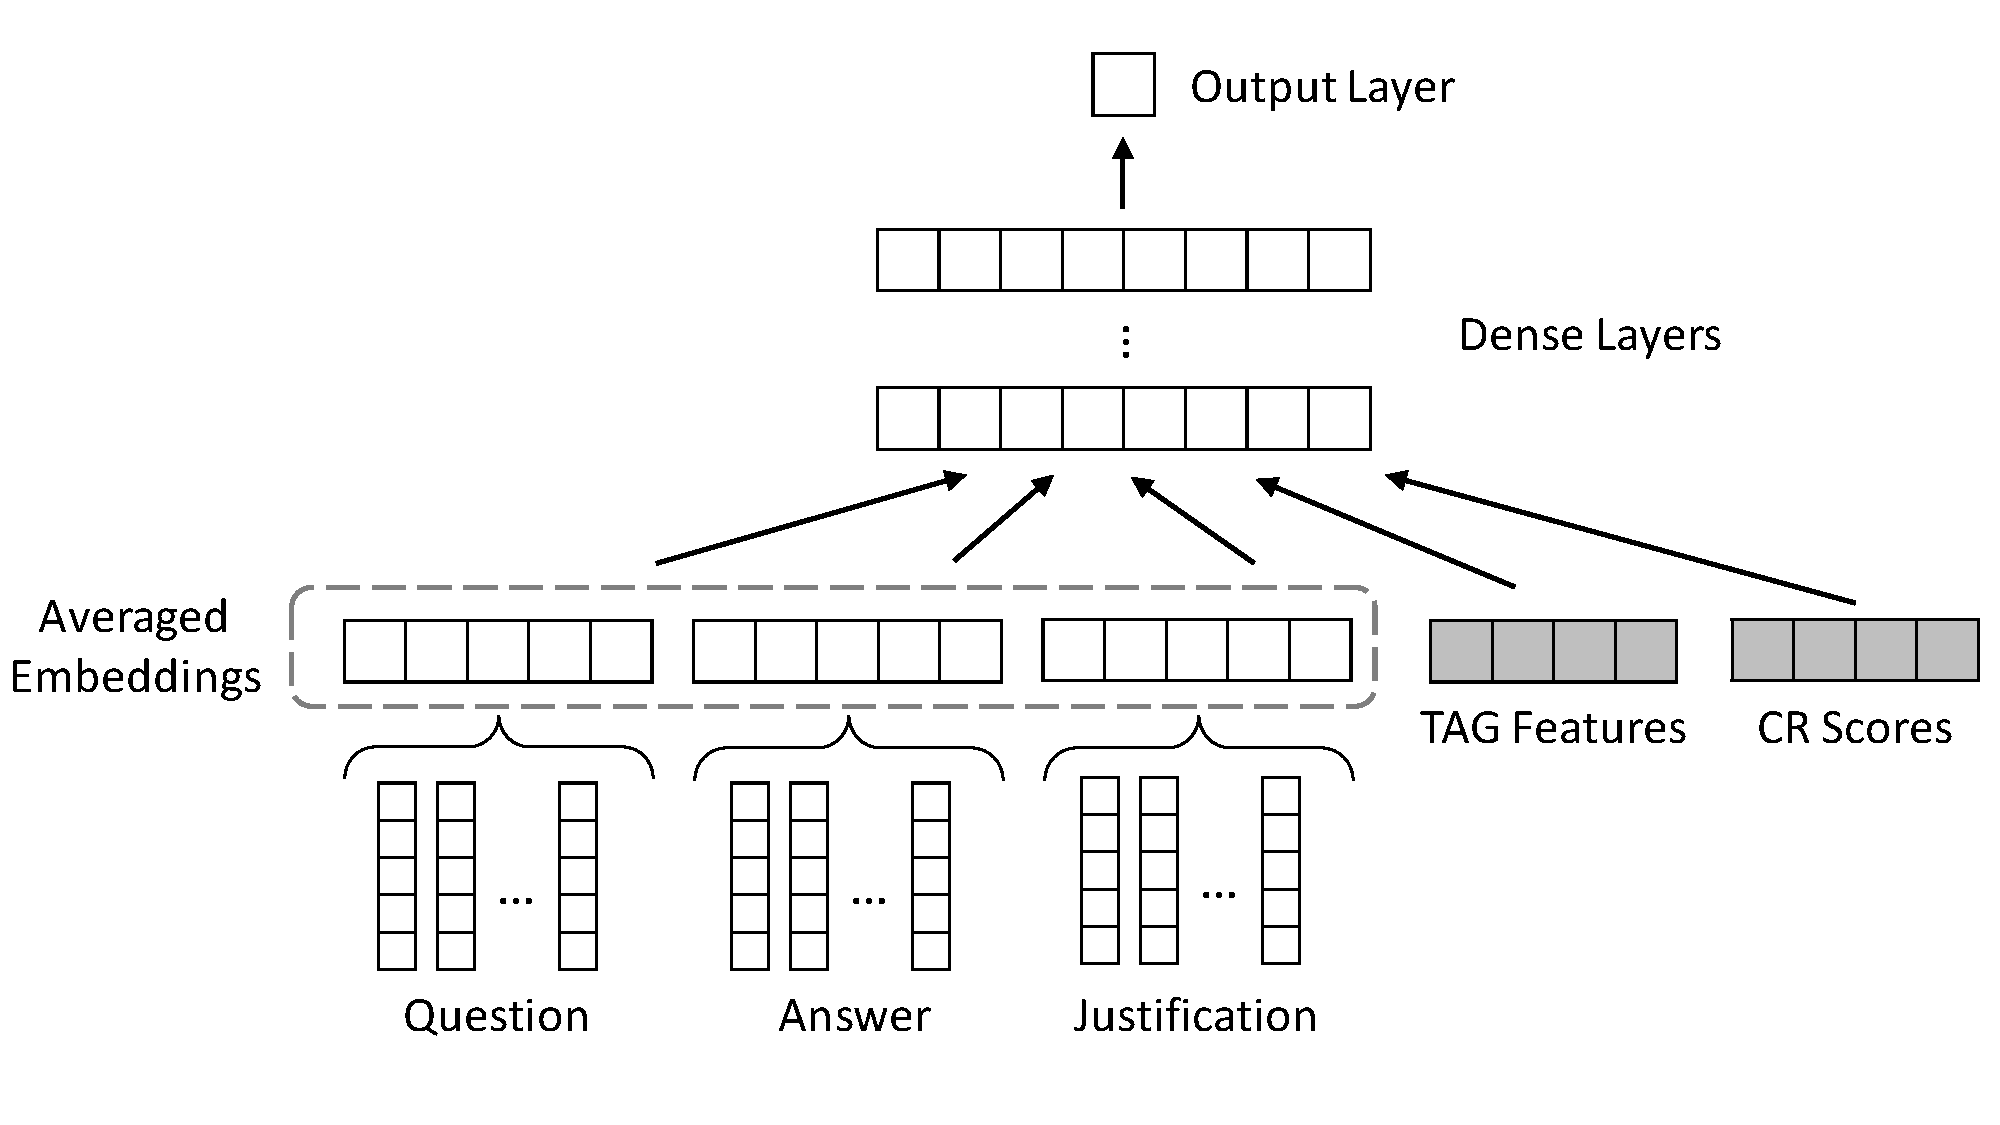
\includegraphics[width=0.8\textwidth]{tagNNArch2scores.pdf}
\caption{The architecture for the neural network variation of our TAG system. We use a fully-connected feed-forward network which takes as input the content words (i.e., nouns, verbs, and adjectives) from the question, candidate answer, and corresponding justification.  For each of these, we create a composite vector by averaging the embeddings of the individual words.  We then concatenate these three composite vectors, as well as the TAG features and the CR scores, to form the input layer to the network. The output of the network is a single, real-valued score for the candidate answer justification.}
\label{fig:nn_arch}
\end{figure}

\subsection{From Latent Perceptron to Latent Neural Networks}
\label{sec:nn}

Neural networks (NNs) have recently received much attention in many NLP tasks and have been shown to be quite effective in certain question answering tasks~\cite{Iyyer2014,bordes2014question,bordes2015large,Iyyer2015,wang2015long,dong2015question,yih2015semantic,he2016pairwise,suggu2016deep}.  To determine if a deep learning approach would benefit our system, we explored providing our text aggregation graph features and the candidate retrieval scores to a neural ranking architecture.  Under this framework we were also able to straightforwardly experiment with including vectorized representations (i.e., embeddings) of the question, candidate answer, and corresponding justification, in hopes of accommodating some of the lexical variation in natural language.

Neural network systems have varied dramatically in terms of their primary architecture (i.e., feed-forward, convolutional, recurrent, etc.) as well as their shape (number of hidden layers, number of nodes in a given layer, etc.).  Recently, however, Iyyer et al.~\citeyear{Iyyer2015} found that in their QA task, a simple network which \emph{averaged} the word embeddings of the questions and the answer candidates outperformed a much more complex tree recurrent NN.  
Chen and Manning \citeyear{chen2016acl} have recently validated this observation in a different QA task.
We based our NN on this simpler system, adapting it to our task by including not only an averaged vector for the question and answer, but also an averaged vector for the answer justification.  Additionally, we include our connection-type aware structural TAG features (cf., Table \ref{tab:features}) and the candidate retrieval (CR) features in the network input.  The network architecture is shown in Figure \ref{fig:nn_arch}.

For learning, we use the hinge ranking loss function \cite{collobert2011natural} and update using stochastic gradient descent (SGD).  During training, for each question we pair the correct answer candidate with each of the incorrect candidates, creating three pairs.  For each of these pairs, we score both the correct answer candidate and the incorrect answer candidate and then compute the loss:
\begin{equation}
L = \max (0, m - F(q,a_{correct}) + F(q,a_{incorrect}))
\end{equation}
where $F(q,a_{correct})$ is the score of the correct answer candidate, $F(q,a_{incorrect})$ is the score of the incorrect answer candidate, and $m$ is the margin.


There are two important aspects of the proposed architecture:
\begin{enumerate}
\item[a)] The latent layer, i.e., identifying good justifications to use for a given answer, which we implement by modifying SGD to keep track of the latent aspect.  Specifically, to maintain the latent variable aspect of our ranking perceptron in our ranking neural network, we adapt Equation \ref{eq:F} to use a feed-forward pass through the network to determine the score of a given TAG (rather than the inner product of the features and the parameter vector), and continue to use the implementation of $P$ that uses only the TAG with highest score.  In this way, for each pair of candidate answers we have two justifications (one for the correct answer and one for the incorrect), and so perform a model update (i.e., backpropagation) for each.
\item[b)] The combination of embeddings with explicit features that come from the CR system and the TAG features.  This strategy of mixing latent and explicit features has been demonstrated to be successful in other NLP tasks \cite{chen2014fast,suggu2016deep}.
\end{enumerate} 

Despite their advantages, neural networks have many hyperparameters which need to be tuned.  Continuing the inspiration of Iyyer et al.~\citeyear{Iyyer2015}, we lightly turned the network on development, both in terms of network shape as well as additional parameters.  Doing so, we arrived at a network which has a single dense layer with length 100 followed by the output layer of length one.\footnote{We experimented with some deeper networks and several hidden layer sizes (both larger and smaller).} 
For our word embeddings, we used a recurrent neural network language model (RNNLM) \cite{mikolov10,mikolov13} trained over a concatenation of all of our in-domain elementary science resources (i.e., the study guides, flashcards, and dictionaries) to generate embeddings with 200 dimensions.\footnote{We also experimented with using embeddings trained over English Gigaword \cite{graff2003english} since the resource is much larger and would potentially yield more robust word representations.  However, we found that the performance was consistently worse, which we suspect is due to the difference in the domains.}  


All network nodes use the sigmoid activation function, which performed better and was more stable to variations in the hyperparameters than the rectified linear unit activation.  Additionally, we used an L2 regularization of 1.0 and a dynamic learning rate which began at 1.0 and decayed by half each time the performance on validation decreased.  Though we experimented with dropout, there did not not seem to be a consistent improvement, so our final models do not include it.    
We used 50 epochs for training with early stopping if the validation performance decreased and failed to regain its previous best after 10 epochs.  Similar to the perceptron, we found that the network performance varied with the random seed.  To mitigate the effects of this variation, we report scores from an ensemble of five networks, each with a different random seed, where the trained networks each voted for a single answer choice, splitting their vote only in the event of a tie.


\begin{table*}
\small
\begin{center}
\caption{Performance of the Latent Ranking Neural Network models.  Models with \emph{CR} include the candidate retrieval scores as input, models with \emph{TAG} use the features from the best performing TAG model (1G\textsubscript{CT}+2G\textsubscript{CT}), and models with \emph{embeddings} include an average embedding for each of the question, the answer, and the text from which the justification graphlet was derived.  Significance tests were performed using bootstrap resampling with 10,000 iterations, but none of the differences between the neural network models and the CR baseline were significant.}
\begin{tabular}{p{0.3mm}p{45mm}ll}
%\multicolumn{1}{l}{ } & \multicolumn{1}{l}{ } & \multicolumn{1}{l}{ } & \multicolumn{1}{l}{P@1}  & \multicolumn{1}{l}{MRR} \\

\# & Neural Network Models  & P\@1 & MRR   \\
% IR - 40.74
% IR + CL + embed - 41.82
% IR + embed - 38.1
% IR + CL - 40.52
% CL - 39.72

\hline
1 & CR				&  40.74\%  & 62.56\%  \\
2 & CR + TAG 		&  40.52\%  & 62.48\% 	\\
3 & CR + embeddings		&  38.74\%  & 61.61\%  	\\
4 & CR + TAG + embeddings	&  41.82\%  & 63.11\%	\\
\end{tabular}
\vspace{-6mm}
\label{tab:nnresults}
\end{center}
\end{table*}

\paragraph{Neural Network Results}
\label{sec:nnresults}


The final performance for the neural network variants of our proposed system as well as the CR baseline are shown in Table \ref{tab:nnresults}.  Once again, we observe that the performance of the combined model (CR + TAG + embeddings, line 4) is better than the performance of the CR model by itself (line 1) or CR + embeddings (line 3). However, here this difference is not significant.  This suggests that representing the justification as a simple bag of words with latent feature representations is not as effective as representing them with features derived from the structure of the text aggregation graph, even with the non-linear capabilities of the neural network.

Additionally, we find that the neural network variants perform worse overall than the latent ranking perceptron models and the voting ensemble (cf., Table \ref{tab:combinedmodels}).  This could be due to the fact that the TAG and CR features we are supplying to the neural network are already abstracted many levels from raw text inputs, and so the NN approach benefits less from the non-linearity of the NN.  Another likely reason for the NN performing worse than the perceptron is that neural architectures need larger quantities of training data in order to properly generalize.  Notably, in the recent Allen Institute for Artificial Intelligence Kaggle challenge\footnote{\url{https://www.kaggle.com/c/the-allen-ai-science-challenge}}, a large contest with 170 participating teams, which also required answering multiple choice elementary and middle school science questions, none of the top-performing participants obtained better results with neural networks. The participants' analyses suggested that this is largely due to a lack of training data.  Finally, the space of possible neural network architectures is large, and the network we report here is fairly simple.  While it could be the case that given a more complex architecture (i.e., with a recurrent or convolutional network, optimizers, and learned rather than pre-trained embeddings) we could obtain even higher numbers than those reported here, with complex architectures, issues resulting from the limited training data would likely be worsened. We leave that exploration to future work.

\paragraph{Incorporating Embeddings into the Perceptron}
Though the embedding-based neural architecture (as implemented) was not successful, following a reviewer suggestion we also experimented with adding the precomputed text embeddings as additional features for the latent ranking perceptron.  In this way, the feature vector for each TAG, $\Phi(x)$, contains the original features as well as an averaged embedding for each of the question, answer, and justification texts.  This provides an additional 600 features, as we are using 200-dimensional embedding vectors.  We included these extra features in our best performing single TAG model, the connection-type aware 1G+2G model shown in Table \ref{tab:combinedmodels}, line 5.  The resulting model performed worse (39.36\% P@1 compared to 42.88\% P@1 without the embeddings). 
This shows that, while distributed representations of words have many benefits (including robustness to lexical variation), their incorporation into a learning model is not necessarily trivial, and we leave that study to future work.

%\begin{table}[!th]
%\begin{center}
%\begin{footnotesize}
%\hfill
%\begin{tabular}{ll}
%\hline
%Error Type & Percent \\ 
%\hline
%Short justification/High lexical overlap  & 53.3\%\\
%Complex inference required   & 43.3\% \\
%Knowledge Base Noise  & 6.7\% \\
%Word order necessary	 & 6.7\% \\
%Coverage & 6.7\% \\
%Negation	& 3.3\% \\
%Other & 6.7\% \\
%\end{tabular}
%\end{footnotesize}
%\caption{{\footnotesize Summary of the findings of the 30 question error analysis.  
%%Examples of several categories provided in separate tables. 
%Note that a given question may fall into more than one category.}} 
%\label{tab:erroranalysis}
%\vspace{-5mm}
%\end{center}
%\end{table}


%\begin{table}[t]
%\begin{center}
%\begin{footnotesize}
%\begin{tabular}{p{1cm}p{6cm}}
%\hline
%Type: & \textbf{Short justification/High lexical overlap}\\
%\hline
%Question: & The length of time between night and day on Earth varies throughout the year. This time variance is explained primarily by $\rule{1cm}{0.15mm}$. \\
%Correct: & Earth 's angle of tilt \\
%			 & \textit{ ... the days are very short in the winter because the sun's rays hit the earth at an extreme angle ... due to the tilt of the earth's axis. } \\
%Chosen: &  Earth 's distance from the Sun \\
%			& \textit{ Is light year time or distance? Distance}	\\
%\end{tabular}
%\hfill
%\end{footnotesize}
%\caption{{\footnotesize Example of the system preferring a justification for which all the terms were found in either the question or answer candidate. (Justifications shown in italics)
%}} 
%\label{tab:ex_lex_overlap}
%\vspace{-5mm}
%\end{center}
%\end{table}

\subsection{Error Analysis}
\label{sec-emnlp2017:erroranalysis}

We performed an error analysis of 30 incorrectly answered questions, %summarized in Table \ref{tab:erroranalysis},
  examining the top 5 justifications returned for both the correct and chosen answers of each.    
%Among the questions analyzed we found some interesting trends.   
Notably, 50\% of the questions had one or more \emph{Good} justifications. %, but the system incorrectly ranked another answer's justification higher.  
The most common form of error (53.3\%) was due to the system's preference for short justifications with a large degree of lexical overlap with the question and answer choice, %, particularly when the correct answer required more "explanation" to connect the question to the answer.  
% shown by the example in Table \ref{tab:ex_lex_overlap}.  
 %This effect was magnified when the correct answer required more "explanation" to connect the question to the answer.  
suggesting the system has learned that generally many unmatched words are indicative of an incorrect answer.  %While this may typically be true, extending the system to be able to prefer the \emph{opposite} with certain types of questions would potentially help with these errors.  
The second largest source of errors (43.3\%) came from questions requiring complex inference (causal, process, quantitative, or model-based reasoning), demonstrating the difficulty of the question set and the need for systems that can robustly handle a variety of question types.
Aside from these main groups, there were some smaller trends including KB noise, and our system's lack of using word order and recognizing negation.\footnote{A much more detailed error analysis is available, and if this paper is accepted will be included.}
 
% as with the question:%.  For example, to answer the question:
 %\begin{quote}
%\begin{addmargin}[1em]{2em}% 1em left, 2em right 
% \begin{footnotesize}
%  \textit{Q: Mr. Harris mows his lawn ...[and leaves] the clippings on the ground. Which long term effect will this most likely have on his lawn? \\
%  A: It will provide the lawn with needed nutrients.}
% \end{footnotesize}
%%\end{quote}
%\end{addmargin}
%To answer this, you would need to link together: \textit{cut grass left on the ground $\rightarrow$ grass decomposes $\rightarrow$ decomposed material provides nutrients}. 
%These questions constitute a large portion of our errors,   demonstrating not only the difficulty of the question set but also the need for systems that can robustly handle a variety of question types and their corresponding information needs.  

%Aside from these main groups, there were some smaller trends including:  
%7\% of the incorrectly chosen answers actually had justifications which "validated" them due to KB noise, 7\% required word-order to answer (e.g., \emph{X divided by Y} vs. \emph{Y divided by X}), %another 7\% of questions suffered from lack of coverage of the question concept in the knowledge base,
%%(see example in Table \ref{tab:ex_coverage}), 
% and 3\% failed to appropriately handle negation (i.e., questions of the format \emph{Which of the following are NOT ...}). 


% bs: no room: - Negative results?


%\begin{table}[t]
%\begin{center}
%\begin{footnotesize}
%\begin{tabular}{p{1cm}p{6cm}}
%\hline
%Type: & \textbf{Coverage}\\
%\hline
%Question: & Which activity most effectively ensures the proper functioning of osteocytes? \\
%Correct: & consuming mineral-rich foods\\
%			& \textit{ most lipids consumed from food are in the form of triglycerids}	\\	
%Chosen & increasing the respiratory rate 	\\
%			& \textit{ hyperventilation increased respiratory rate}	\\
%\end{tabular}
%\hfill
%\end{footnotesize}
%\caption{{\footnotesize Example of a question for which coverage was an issue.  The KB had no coverage for the concept of \emph{osteocyte}.}} % , so the system grasped at proverbial straws.}} 
%\label{tab:ex_coverage}
%\end{center}
%\end{table}


%\begin{table}[!th]
%\begin{center}
%\begin{footnotesize}
%\begin{tabular}{p{1cm}p{6cm}}
%\hline
%Type: & \textbf{Complex inference required}\\
%\hline
%Question: & Mr. Harris mows his lawn twice each month. He claims that it is better to leave the clippings on the ground. Which long term effect will this most likely have on his lawn? \\
%Correct: &  It will provide the lawn with needed nutrients. 	\\
%\end{tabular}
%\hfill
%\end{footnotesize}
%\caption{{\footnotesize Example of a question for which complex inference is required.  In order to answer the question, you would need to assemble the following chain of events: cut grass left on the ground $\rightarrow$ grass decomposes $\rightarrow$ decomposed material provides nutrients.}} 
%\label{tab:ex_complex_inf}
%\end{center}
%\end{table}


\section{Conclusion}
\label{sec:conclusion}

We have proposed an approach for QA where producing human-readable justifications for answers, and evaluating answer justification quality, is the critical component.
Our interdisciplinary approach to building and evaluating answer justifications includes cognitively-inspired aspects, such as making use of psycholinguistic concreteness norms for focus word extraction, and making use of age-appropriate knowledge bases, which together help move our approach towards approximating the qualities of human inference on the task of question answering for science exams. Intuitively, our structured representations for answer justifications can be interpreted as a robust approximation of more formal representations, such as logic forms~\cite{moldovan2001logic}. However, our approach does not evaluate the quality of connections in these structures by their ability to complete a logic proof, but through a reranking model that measures their correlations with good answers.

In our quest for explainability, we have designed a system that generates answer justifications by chaining sentences together. Our experiments showed that this approach improves explainability, and, at the same time, answers questions out of reach of information retrieval systems, or systems that process contiguous text.  
We evaluated our approach on 1,000 multiple-choice questions from elementary school science exams, and experimentally demonstrated that our method outperforms several strong baselines at both selecting correct answers, and producing compelling human-readable justifications for those answers.  We further validated our three critical contributions: (a) modeling the high-level task of determining justification quality by using a latent variable model is important for identifying both correct answers and good justifications, (b) identifying focus words using psycholinguistic concreteness norms similarly benefits QA for elementary science exams, and (c) modeling the syntactic and lexical structure of answer justifications allows good justifications to be assembled and detected. 

We performed a detailed error analysis that suggests several important directions for future work. 
First, though the majority of errors can be addressed within the proposed formalism and by improving focus word extraction, 47.5\% of incorrectly answered questions would also benefit from more complex inference mechanisms, ranging from causal and process reasoning, to modeling quantifiers and negation.
This suggests that our robust approach for answer justification may complement deep reasoning methods for QA in the scientific domain~\cite{baral2011towards}.
Second, our text aggregation graphs currently capture intersentence connections solely through lexical overlap. We hypothesize that extending these structures to capture lexical-semantic overlap driven by word embeddings~\cite{mikolov13}, which have been demonstrated to be beneficial for QA~\cite{yih13,jansen14,fried2015higher}, would also be beneficial here, and increase robustness on small knowledge bases, where exact lexical matching is often not possible. 
Finally, while our answer justifications are currently short, future justifications might be quite long, and aggregate sentences from knowledge bases of different domains and genres.  In these situations, combining our procedure for constructing justifications with methods that improve text coherence~\cite{barzilay2008modeling} would likely improve the overall user experience for reading and making use of answer justifications from automated QA systems. 

To increase reproducibility, all the code behind this effort is released as open-source software\footnote{\url{https://github.com/clulab/releases/tree/master/cl2017-qa}}, which allows other researchers to use our entire science QA system as is, or to explore adapting the various components to other tasks. 

\FloatBarrier


%\section*{Acknowledgments}

\bibliography{refs}
\bibliographystyle{emnlp_natbib}

\end{document}
